\subsubsection{Experiments for Eliciting Anger Emotion}

To study the emotion of anger across various intensity levels, three custom-designed gameplay tasks were developed. All tasks introduce frustration through interruptions, distractions, or interface issues—elements proven to induce negative emotional responses like anger in controlled experiments.

\paragraph*{Low-Intensity Anger – Chrome Dino Game with Noise Distraction}

The first task involves participants playing the well-known Chrome Dino game. However, to introduce a frustrating element, the game is played while the participant listens to honking vehicle sounds and other urban noise distractions via audio playback (\url{https://www.youtube.com/watch?v=d0k1JFAAMCo}) \citep{soundsforyou_traffic_noise}.

Research has shown that auditory noise, particularly when irrelevant to the task, can significantly interfere with attentional control and lead to feelings of frustration and mild anger~\citep{choi2013audio}. Even non-hazardous noise levels can trigger emotional stress, especially during cognitive tasks. In gaming scenarios, background noise is found to negatively affect concentration and cognitive performance, making it a useful tool to induce low levels of anger or irritation.

\paragraph*{Medium-Intensity Anger – Number Game with Pop-Up Interruptions}

The second task involves a number selection game where participants must click numbers in ascending order under a time constraint. As the game progresses and the participant nears completion, random pop-up ads begin appearing more frequently. In the last 10 seconds, a countdown starts flashing and loud beep sounds are introduced to further stress the player. Ultimately, due to these disruptions, the game becomes unwinnable.

Scientific literature supports the idea that unexpected interruptions such as pop-up ads can be strong triggers for anger and frustration. Such ads are perceived as highly intrusive and break the player's sense of immersion and control~\citep{hanbazazh2021pop}. The psychological theory of reactance further suggests that when individuals feel their freedom to act is restricted (e.g., by pop-ups interfering with gameplay), they experience negative emotions such as frustration and anger. These effects are even more pronounced when the interruptions occur during critical moments, which is intentionally designed in this task.

\paragraph*{High-Intensity Anger – Flappy Bird Variant with Broken Controls}

The third task is based on the classic Flappy Bird game. However, participants are given no instructions on how to play. Furthermore, the game mechanics behave unpredictably: pressing the spacebar does not always trigger a jump, and sometimes causes the window to scroll instead. As in the first task, distracting honking sounds play in the background to further irritate the participant.

This task is designed to provoke a high level of anger by breaking the user’s mental model of how the game should behave. When participants feel they are failing not due to their own skill but because of poor or broken game mechanics, frustration increases dramatically. Studies have shown that unclear game objectives and malfunctioning controls significantly reduce players' sense of competence and autonomy, which are essential psychological needs~\citep{bevilacqua2019game}. When those needs are blocked, it can lead to intense anger and even aggressive reactions, including what’s commonly known as “rage quitting.”

Screenshots related to the anger eliciting tasks are shown in Figure~\ref{fig:task-angry}. The fourth image shows the Chrome Dino game with noise distractions, the fifth image shows the number game with pop-up interruptions, and the last image shows the Flappy Bird variant with broken controls. These tasks were designed to be engaging and varied, ensuring that participants could experience anger at different intensity levels.

\begin{figure*}[h]
    \centering
    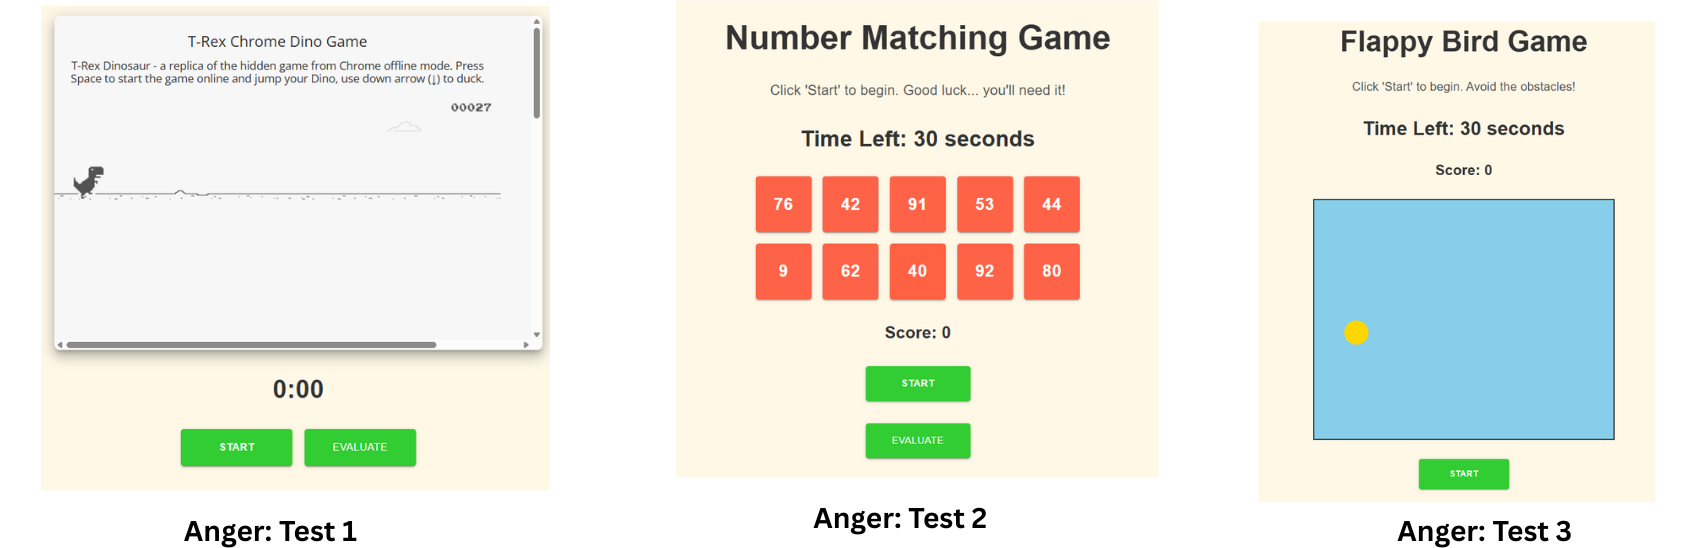
\includegraphics[width=1\textwidth]{img/chapter_03/angry_tests.png}
    \captionof{figure}{Eliciting tasks for Anger Emotion}
    \label{fig:task-angry}
\end{figure*}

